\documentclass[11pt,a4paper]{article}
\usepackage[spanish,es-nodecimaldot]{babel}	% Utilizar español
\usepackage[utf8]{inputenc}					% Caracteres UTF-8
\usepackage{graphicx}						% Imagenes
\usepackage[hidelinks]{hyperref}			% Poner enlaces sin marcarlos en rojo
\usepackage{fancyhdr}						% Modificar encabezados y pies de pagina
\usepackage{float}							% Insertar figuras
\usepackage[textwidth=390pt]{geometry}		% Anchura de la pagina
\usepackage[nottoc]{tocbibind}				% Referencias (no incluir num pagina indice en Indice)
\usepackage{enumitem}						% Permitir enumerate con distintos simbolos
\usepackage[T1]{fontenc}					% Usar textsc en sections
\usepackage{amsmath}						% Símbolos matemáticos
\usepackage[simplified]{pgf-umlcd}
\usepackage{pdflscape}
\usetikzlibrary{babel} % Problemas del español al usar <,> para las citas
\usepackage{typearea} % Paginas horizontales

\usepackage{listings}
\usepackage{xcolor}
 
\definecolor{codegreen}{rgb}{0,0.6,0}
\definecolor{codegray}{rgb}{0.5,0.5,0.5}
\definecolor{codepurple}{rgb}{0.58,0,0.82}
\definecolor{backcolour}{rgb}{0.95,0.95,0.92}
 
\lstdefinestyle{mystyle}{
    backgroundcolor=\color{backcolour},   
    commentstyle=\color{codegreen},
    keywordstyle=\color{magenta},
    numberstyle=\tiny\color{codegray},
    stringstyle=\color{codepurple},
    basicstyle=\ttfamily\footnotesize,
    breakatwhitespace=false,         
    breaklines=true,                 
    captionpos=b,                    
    keepspaces=true,                 
    numbers=left,                    
    numbersep=5pt,                  
    showspaces=false,                
    showstringspaces=false,
    showtabs=false,                  
    tabsize=4,
    language=Java
}
 
\lstset{style=mystyle}

% Comando para poner el nombre de la asignatura
\newcommand{\asignatura}{Nuevos Paradigmas de Interacción}
\newcommand{\autorv}{Vladislav Nikolov Vasilev}
\newcommand{\autorj}{José María Sánchez Guerrero}
\newcommand{\autorf}{Fernando Vallecillos Ruiz}
\newcommand{\titulo}{Práctica Sensores}
\newcommand{\subtitulo}{Memoria Técnica}


% Configuracion de encabezados y pies de pagina
\pagestyle{fancy}
\lhead{Vladislav, José María, Fernando}
\rhead{\asignatura{}}
\lfoot{Grado en Ingeniería Informática}
\cfoot{}
\rfoot{\thepage}
\renewcommand{\headrulewidth}{0.4pt}		% Linea cabeza de pagina
\renewcommand{\footrulewidth}{0.4pt}		% Linea pie de pagina


% new pagestyle
\fancypagestyle{lscape}{
  \headwidth\textwidth
}

\begin{document}
\pagenumbering{gobble}

% Pagina de titulo
\begin{titlepage}

\begin{minipage}{\textwidth}

\centering

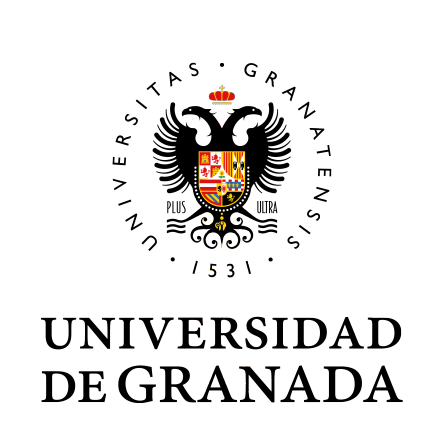
\includegraphics[scale=0.5]{img/ugr.png}\\

\textsc{\Large \asignatura{}\\[0.2cm]}
\textsc{GRADO EN INGENIERÍA INFORMÁTICA}\\[1cm]

\noindent\rule[-1ex]{\textwidth}{1pt}\\[1.5ex]
\textsc{{\Huge \titulo\\[0.5ex]}}
\textsc{{\Large \subtitulo\\}}
\noindent\rule[-1ex]{\textwidth}{2pt}\\[3.5ex]

\end{minipage}

\vspace{0.5cm}

\begin{minipage}{\textwidth}

\centering

\textbf{Autores}\\ {\autorv{}}\\{\autorj{}}\\{\autorf{}}\\[2.5ex]
\textbf{Rama}\\ {Computación y Sistemas Inteligentes}\\[2.5ex]
\vspace{0.3cm}


\includegraphics[scale=0.3]{img/etsiit.jpeg}

\vspace{0.5cm}
\textsc{Escuela Técnica Superior de Ingenierías Informática y de Telecomunicación}\\
\vspace{0.5cm}
\textsc{Curso 2019-2020}
\end{minipage}
\end{titlepage}

\pagenumbering{arabic}
\tableofcontents
\thispagestyle{empty}				% No usar estilo en la pagina de indice

\newpage

\setlength{\parskip}{1em}


\section{Introducción}
En este proyecto vamos a explicar nuestra \textit{Natural User Interface (NUI)} que hará que nuestra visita a la Alhambra sea más
dinámica y productiva. El proyecto constaría de varios dispositivos, como pueden ser principalmente unas gafas de realidad aumentada,
un dispositivo \textit{Leap Motion} y un micrófono integrados en las gafas, y un \textit{smartphone} que utilizaremos tanto para
manejar el sistema gracias a los múltiples sensores que incorpora como para controlar la aplicación.

En esta segunda versión del proyecto vamos a encargarnos de la interfaz por gestos, es decir, dejaremos a un lado los sensores
y el controlador por voz. Vamos a encargarnos de la realidad aumentada y los gestos para manejar el sistema.

\section{Interfaz por gestos}
Como no disponemos de unas gafas con un Leap Motion incorporado, vamos a realizar nuestra simulación en un programa de python aparte. En
nuestra versión, la opción de utilizarlo verticalmente no está disponible, por lo que su funcionamiento se mostrará con el dispositivo
sobre la mesa. Implementaremos los gestos $click$, $swipe$, zoom y agarre y movimiento, que explicaremos a continuación:

\subsection{Descripción del \textit{click}}
Este gesto servirá para mostrar la información extra del objeto. El gesto consiste en cerrar y abrir el puño en la zona sobre la que
queremos obtener la información. Esta zona se detectaría automáticamente con un algoritmo implementado en las gafas, pero como no disponemos
de esta tecnología, utilizaremos una imagen fija con una zona resaltada en nuestra simulación.

Esto mostrará en la interfaz de nuestras gafas de realidad aumentada una imagen de la zona resaltada, junto con información de esta. Esta
información podrá ser modificada mediante otros gestos descritos posteriormente.

La implementación de este gesto es la siguiente:





\subsection{Descripción del \textit{swipe}}
Al igual que mostramos la información con el gesto anterior, necesitaremos otro gesto para ocultarla. Nosotros utilizamos el $swipe$, el cual
detectará los movimientos en el eje X, así podrá usarse tanto para diestros como para zurdos. Modificaremos el parámetro de su velocidad
para que no se pueda confundir con otros gestos que hacemmos naturalmente.

La implementación es la siguiente:

implemetasion

cosass extra


\subsection{Descripción del zoom}
Este gesto sirve para disminuir o aumentar el tamaño de la información mostrada. Para utilizar este gesto tendremos que tener las dos manos
sobre la zona de detección del $Leap Motion$ y, posteriormente, extender los dedos pulgar e índice con una apertura mínima entre ellos de 40º.
El zoom que se le aplicará a la imagen será directamente proporcional a la distancia en el eje X entre la mano derecha y la mano izquierda.

implemetasion



cosass extra
Además de hacer zoom, también está implementada una función que, si llegamos a un umbral de zoom en algunas zonas determinadas (por ejemplo,
a la fuente de la funete de los leones, o una habitación del Palacio de Carlos V), mostraremos información más detallada sobre ésta. La
implementación es la siguiente?? o ya la hemos puesto antes???


\subsection{Descripción del agarre y movimiento}
Para mover la información sobre toda la superficie de las gafas de realidad aumentada, utilizaremos el siguiente gesto. Cerraremos el puño
(tendrá que ser en las mismas coordenadas sobre las que está la información, para así evitar moverla sin querer con algún gesto natural) y
posteriormente la moveremos al lugar que queramos. Para dejar de moverla, simplemente volvemos a abrir la mano.

Si estamos arrastrando la información fuera de nuestro campo de visión, hemos puesto unos límites tanto vertical como horizontalmente, para que
el programa no nos permita hacerlo.

Arrastrada la información, también guardaremos las propiedades que conservaba previamente, como por ejemplo, si le habíamos hecho zoom, o la
habíamos arrastrado en otro momento.

implemetasion

cosass extra

\newpage

\begin{thebibliography}{5}

\bibitem{bib:permisos}
Permisos en Android
\\\url{https://developer.android.com/reference/androidx/core/app/ActivityCompat.html#requestPermissions(android.app.Activity,%20java.lang.String%5B%5D,%20int)}

\bibitem{bib:fragment}
\textit{Fragment} en Android
\\\url{https://developer.android.com/reference/android/app/Fragment#onCreateView(android.view.LayoutInflater,%20android.view.ViewGroup,%20android.os.Bundle)}

\end{thebibliography}

\end{document}

